\section{Eksempel på IoT angreb}
En kilde \autocite{UCBerkeley} har lavet et studie, hvor de kigger på hvordan kan finde og styre IoT-enheder på et LAN netværk uden selv at være en del af LAN netværket. Studiet erkender at der er flere måder at overtage kontrollen af en IoT-enhed på. Den direkte måde er hvis enheden er åben ud til internettet altså at den har en web-frontend som er tilgængelig for alle. Hvis det er tilfældet, så skal der kun en svaghed til før at angriberen har overtaget enheden. Enheder som disse er ofte ganske enkle at finde frem til, f.eks. kan søgemaskinen Shodan bruges til at finde enheder af bestemte mærker der hoster servere udadtil.\\
Det scenarie som studiet kigger på, er hvor IoT-enheden ikke direkte kan tilgås fra internettet og dermed skulle man tro at den er sikret for angreb. Artiklen beskriver, hvordan at de kan overtage IoT-enheden fra en browser på en computer over LAN netværket.
De starter med enten at lave en hjemmeside som indeholder ondsindet kode som en browser eksekvere når computeren besøger hjemmesiden, eller benytte et \gls{cross_site_scripting} angreb til at få den ondsindede kode til at køre på en troværdigt website. Koden udnytter offerets browser til at søge efter IoT-enheder på LAN netværket og identificere, hvilke enheder der er på netværket. Det kan lade sig gøre da koden er javascript, som eksekveres client-site, altså lokalt på brugerens computer i modsætning til f.eks PHP som eksekveres på webserveren. På denne måde undgår scriptet at skulle igennem routeren's firewall, som ellers normalt giver en del beskyttelse mod angreb udefra.
Javascript koden kan gøre det ved at sende en kommando til IP-adressen på en ubrugt port. Hvis der ikke er nogen enhed på IP-adressen, så kommer der ikke noget svar tilbage, men hvis der er en enhed så får man ofte et svar. Ud fra svaret vil det ofte være muligt at afgøre hvilken enhed der er på IP-adressen fx en chromecast.\\
    \begin{figure}[H]
        \centering
            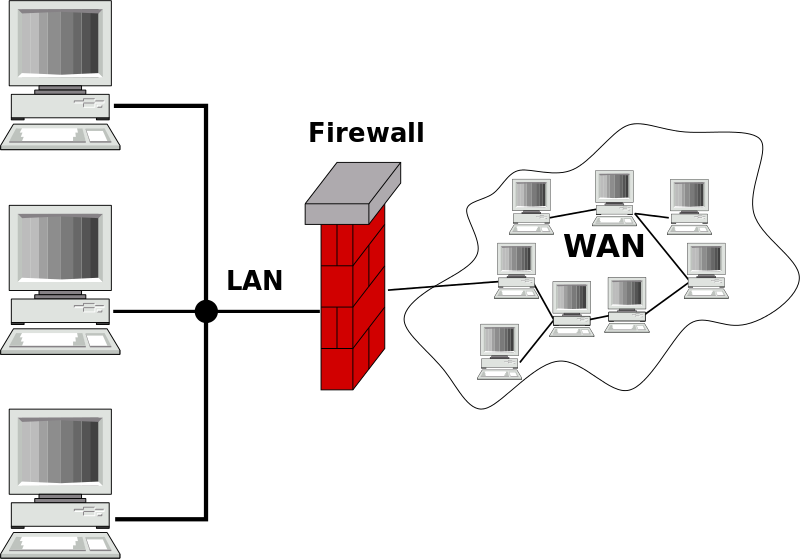
\includegraphics[width=0.7\textwidth]{figures/800px-Gateway_firewall.png}
        \caption{En router's firewall beskytter mod angreb udefra, men ikke fra andre enheder på LAN netværket\label{fig:updates}}
    \end{figure}
Næste trin er hjemmesiden prøver at udføre et \Gls{DNS_rebinding} angreb, gennem browseren, på IoT-enheden. Det betyder at browseren først forbinder til den ondsindede hjemmeside hvor kode køres på computeren. Koden venter nu til at det lagerede data i browseren skal opdateres, da det er blevet for gammelt og denne gang giver hjemmesiden nu en ny DNS IP-adresse, som er en lokal adresse tilhørende en IoT-enhed. Nu kan der sendes kommandoer til IoT-enheden uden at sikkerheden opdager det. Det vil sige at nu er IoT-enheden overtaget og der kan sendes og modtages data til og fra enheden. I dette angreb benyttes simple HTTP requests som \Gls{GET} og \Gls{POST} til at enten hente information fra de forskellige enheder, eller sende kommandoer til dem. Informationen der kan hentes inkluderer i mange tilfælde ting som software og firmware version samt model detaljer. Alle disse er enormt brugbare, hvis man vil tage fuld kontrol over enhederne til f.eks. et \gls{botnet}, da firmware og software version er essentielle når det kommer til at finde sårbarheder, der virker mod den specifikke enhed. Kommandoerne der kunne sendes varierede meget i artiklens eksempel, nogle enheder som Chromecast og et Smart-TV kunne afspille videoer, mens en enkelt enhed med \Gls{POST} requests gav fuld kontrol over al dens funktionalitet.
Computer med browseren der har besøgt den ondsindede hjemmeside er på intet tidspunkt blevet overtaget, da browseren beskytter sådan et angreb. Problemet er nu at IoT-enheden, som er overtaget, kan tilgå computeren over LAN netværket og på den måde er computeren ikke længere i sikkerhed.
\\
Angrebet virker kun hvis IoT-enheden bruger HTTP til dens hjemmeside interface og der ikke er en alt for kompleks kode. Det kræves selvfølgelig også at den svare på beskeden på den ubrugte port, hvis ikke den gør det er første del af angrebet ikke muligt. Browseren skal også tillade de forskellige kommandoer angrebet kræver for at lykkedes. Der er mange ændringer der kan laves for at sådan et angreb ikke længere er mulige. Det er dog vigtigt at huske, at dette langt fra er den eneste måde hvorpå ondsindede typer, kan få adgang til dine IoT enheder, så det at fikse en af de overstående parametre, vil ikke være nok til at sikre din IoT enhed komplet.
\\